Audio restoration has gained widespread application across various scenarios, ranging from music playback to real-time communication systems. For instance, in restoring vintage music, audio restoration methods effectively rejuvenate classic music pieces eroded by time or constrained by outdated equipment \cite{lattner2021stochastic,liu2021voicefixer}. Moreover, these methods are found to be extensively used in speech communication, particularly in telephone or internet calls, by repairing low-quality or distorted codec audio at the receiving end, thereby delivering a clearer and more natural auditory experience \cite{deng2020exploiting,dietz2002spectral,backstrom2017speech,li2024audio}. In music playback, audio restoration mitigates the degradation caused by compression, ensuring that users enjoy high-fidelity audio \cite{deng2020exploiting,lemercier2024diffusion,moliner2023solving}. For generative models, such as those used in music generation and speech synthesis, the audio quality is crucial, and restoration methods can enhance data quality, thus significantly improving model performance \cite{ji2020comprehensive,uhlich2024sound}. Robust audio restoration methods have become indispensable components of modern audio processing systems.

Audio restoration involves predicting high-quality, undistorted audio from degraded or compressed inputs. Current audio restoration technologies primarily focus on vocal recovery \cite{deng2020exploiting,dietz2002spectral,backstrom2017speech}. In traditional methods, a common technique is bandwidth extension \cite{dietz2002spectral,backstrom2017speech}, which aims to reconstruct lost high-frequency information and improve the perceptual quality of highly compressed audio signals. High-frequency spectral extension enhances encoding efficiency and proves crucial in low-bitrate scenarios \cite{larsen2005audio}. However, in some cases, bandwidth extension can introduce high-frequency artifacts that may degrade the overall audio signal quality.

\begin{figure*}[h]
	\small
	\centering
	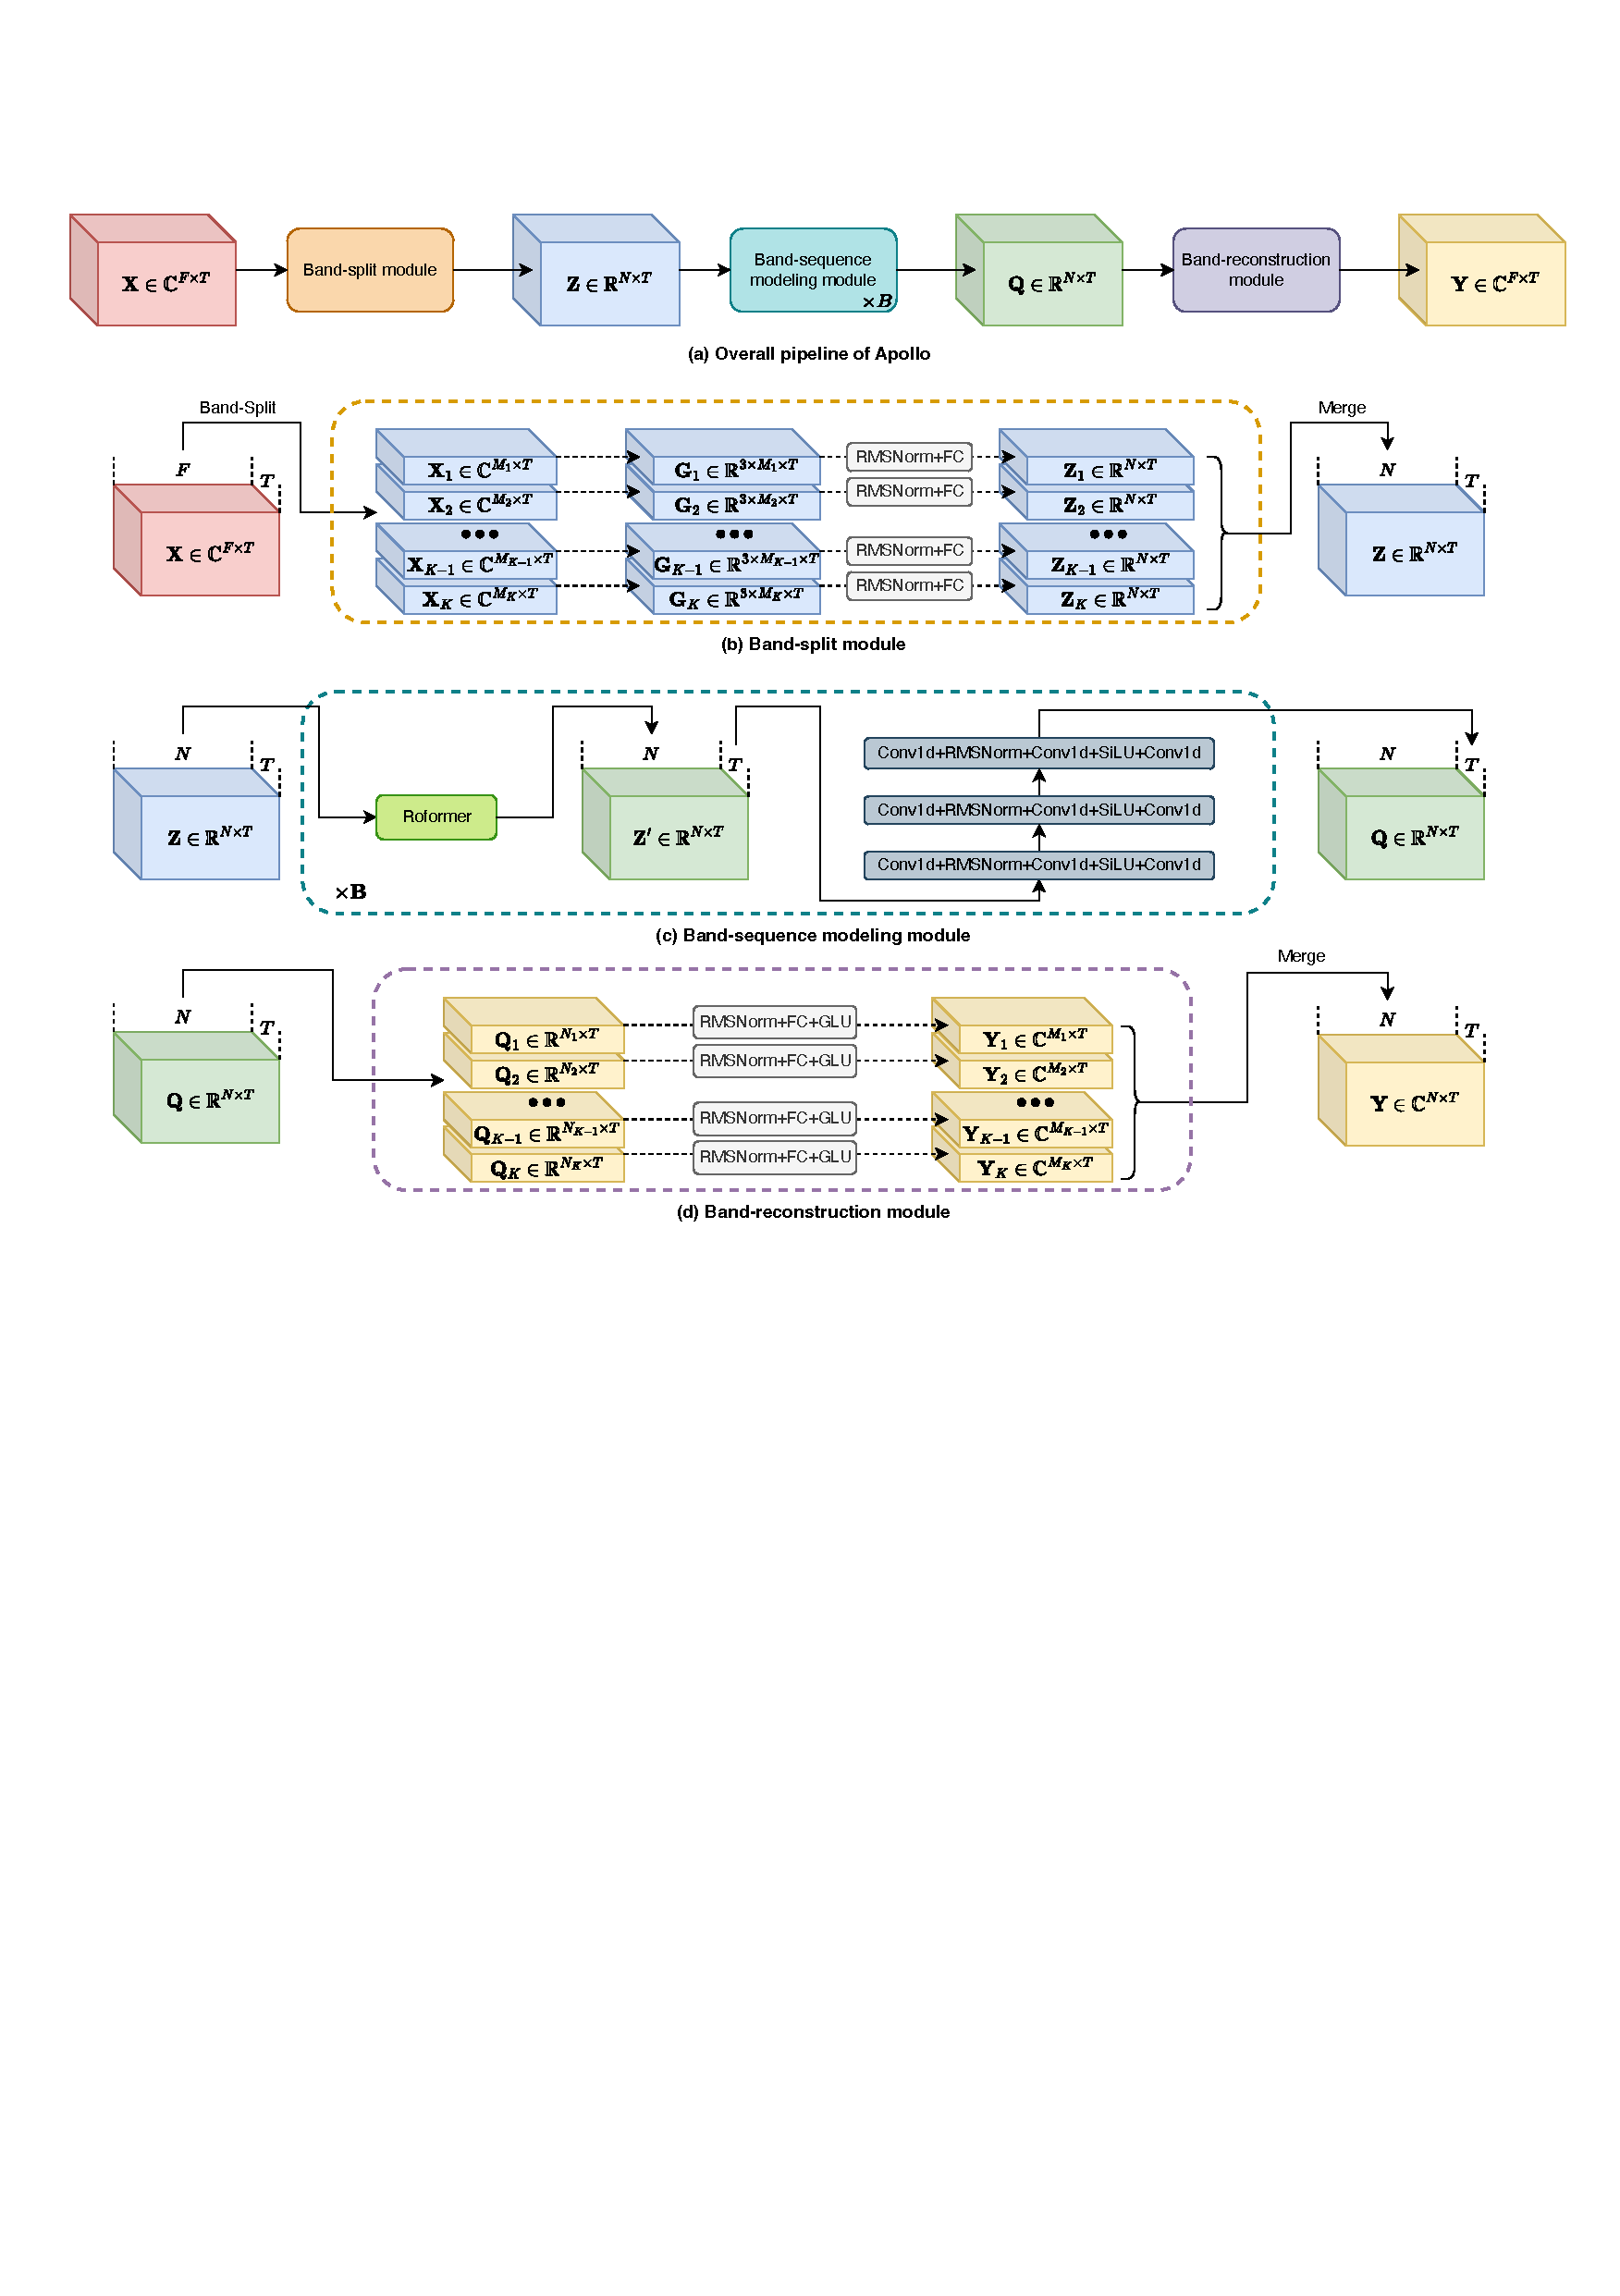
\includegraphics[width=2.0\columnwidth]{Figures/refiner.pdf}
	\caption{Overall pipeline of the model architecture of Apollo and its modules.}
	\label{fig:refiner}
\end{figure*}

With the rapid advancement of deep learning, NN-based methods have gradually replaced traditional signal-processing methods. Recently, GANs \cite{goodfellow2020generative} have demonstrated substantial potential in audio super-resolution and restoration tasks \cite{lattner2021stochastic,pascual2017segan}, especially in achieving high-quality restoration. In audio codecs \cite{wu2023audiodec,kumar2024high,luo2024gull}, GANs effectively balance perceptual audio quality with distortion, offering superior restoration performance compared to traditional methods. Audio degradation typically affects the mid-to-high-frequency bands, particularly when using lossy codecs such as MP3 or AAC \cite{brandenburg1999mp3}, where high-frequency information is prone to compression artifacts. An ideal generator should retain the original audio's low-frequency components and supplement smooth and delicate mid-to-high-frequency details, thereby achieving a more realistic audio restoration effect. The Gull codec \cite{luo2024gull} has successfully demonstrated the effectiveness of GANs in the audio codec, showing significant progress in the super-resolution reconstruction of music and speech during the decoding phase of lossy codecs.

Inspired by Gull, we propose the Apollo model, a generative model specifically designed for high-sampling-rate audio restoration tasks. Apollo supports restoring audio quality at different compression rates. It comprises three main modules: a frequency band split module, a frequency band sequence modeling module, and a frequency band reconstruction module. Unlike Gull, we employ Roformer \cite{su2024roformer} in the frequency band sequence modeling module to capture frequency features and use TCN to model temporal features, enabling more efficient audio restoration. Specifically, Apollo first divides the spectrogram into sub-band spectrograms with predefined bandwidths, extracts gain-shape representations for each sub-band spectrogram, and encodes them through a bottleneck layer. Subsequently, stacked frequency band-sequence modeling modules perform interleaved modeling across frequency bands and sequences. Finally, each sub-band feature is mapped through nonlinear layers to generate the estimated restored sub-band spectrogram. These modules' design ensures the preservation of low-frequency information while restoring high-quality mid and high-frequency components. Additionally, with causal convolution and causal Roformer, our model supports streaming processing, making it suitable for real-time audio restoration.

We evaluated Apollo on the MUSDB18-HQ \cite{rafii2019musdb18} and MoisesDB \cite{pereira2023moisesdb} datasets, comparing it with state-of-the-art models such as SR-GAN \cite{lattner2021stochastic}. The experimental results showed that Apollo performed exceptionally well across various compression bitrates and music genres, particularly in complex scenarios involving a mixture of multiple instruments and vocals. Additionally, Apollo's efficiency in streaming audio applications has been validated, demonstrating its potential in real-time, high-quality audio restoration.